\documentclass[tikz, border=2pt]{standalone}
\usepackage{tikz}
\usepackage{pgfplots}
\usetikzlibrary{decorations.pathreplacing,calc}
\begin{document}
    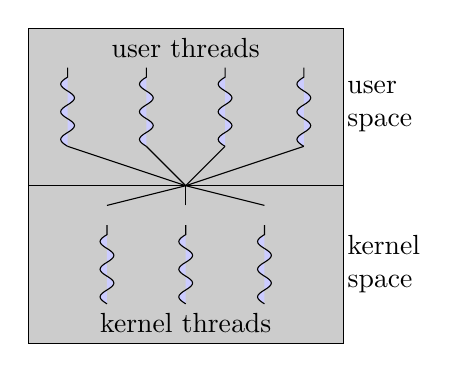
\begin{tikzpicture}
        \draw [fill=black!20] (0.5,0.5) rectangle (4.5,2.5);
        \draw [fill=black!20] (0.5,2.5) rectangle (4.5,4.5);
        \foreach \x in {1,...,4}
        {
            \draw[fill=blue!20, decorate, decoration={coil,aspect=0}] (\x,3) -- (\x,4);
            \draw (\x,3) -- (2.5,2.5);
        }
        \foreach \x in {1.5,...,3.5}
        {
            \draw[fill=blue!20, decorate, decoration={coil,aspect=0}] (\x,1) -- (\x,2);
            \draw (\x,2.25) -- (2.5,2.5);
        }
        \node [below, align=center] at (2.5,1) {kernel threads};
        \node [above, align=center] at (2.5,4) {user threads};
        \node [left, align=left] at (5.5,3.5) {user\\space};
        \node [left, align=left] at (5.6,1.5) {kernel\\space};
    \end{tikzpicture}
\end{document}